\makeatletter
\def\input@path{{../}}
\makeatother
\documentclass[../main.tex]{subfiles}
\begin{document}
\renewcommand{\path}{3_chapter_1/}
\chapter[Toy Modelling for teaching and developing Methodology]{Using simple Models to understand and develop Methodology - Ensembler
    \footnote{\label{footnoteChapter1CopyRight} 
    Reprinted (adapted) with permission from Benjamin Ries, Stephanie M. Linker, David F. Hahn, Gerhard König and Sereina Riniker ,
    J. Chem. Inf. Model., \textbf{61}, 560-564 (2021). Copyright 2021 American Chemical Society.}
}
\chaptermark{FE: Toy Modelling}
\label{ch:feens}

\aquote{
"It all works because Avogadro's number is closer to infinity than to 10."
}{R. Baierlein\\ Gromacs quote collection \cite{Abraham2015}}




\begin{summary}
Ensembler is a python package that allows for fast and easy access to the simulation of one and two-dimensional model systems.
It enables method development using small test systems and to deepen the understanding of a broad spectrum of molecular dynamics (MD) methods, starting from basic techniques to enhanced sampling and free-energy calculations.
The ease of installing and using the package increases shareability, comparability, and reproducibility of scientific code developments.
Here, we provide a description of the implementation and usage of the package as well as an application example for free-energy calculation.
The code of Ensembler is freely available on GitHub \textit{https://github.com/rinikerlab/Ensembler}.
%
\end{summary}

\clearpage
\pagebreak

%%%%%%%%%%%%%%%%%%%%%%%%%%%%%%%%%%%%%%%%%%%%%%%%%%%%%%%%%%%%%%%%%%%%%
%% Start the main part of the manuscript here.
%%%%%%%%%%%%%%%%%%%%%%%%%%%%%%%%%%%%%%%%%%%%%%%%%%%%%%%%%%%%%%%%%%%%%
%================================================================================
\section{Introduction}
%================================================================================

%The Problem and the Solution
Newly developed advanced simulation methods are routinely tested on simple one- and two-dimensional model systems. They provide valuable insights into the theory, conceptual advantages and limitations (for examples see e.g. Refs. \cite{Huber1994, Laio2002, Christ2007, Konig2012, Koenig2020, Donnini2016, Weiss2016, Lemke2018}).
While the results of new methods are published, the implementation details may not always be available or difficult to use with different computer infrastructure.
As a result, sharing, reproducing, understanding, and comparing simulation methodologies is often cumbersome.\cite{Peng2011}
To address this issue, we have developed the Ensembler package, an easy-to-use, yet powerful platform that enables fast prototyping of new methods and comparison against existing techniques using one or two-dimensional test systems.

%Global ethical goal
Ensembler is designed following the recommendations of Stodden \textit{et al.}\cite{Stodden2016} for the enhanced reproducibility of computational methods, which includes making code publicly accessible, providing documentation, and using open licensing.\cite{Stodden2016} 
Furthermore, Ensembler uses state-of-the-art software engineering tools (i.e. git,\cite{Chacon2014} MolSSI cookie-cutter,\cite{Naden2018} and binder\cite{Binder2018}/Colab\cite{Bisong2019}) to fulfill these recommendations and enable features like continuous integration and the transparent versioning of the code. 

%-------------------------------------------------------------------------------------------------------
\subsection{Method Development}
%-------------------------------------------------------------------------------------------------------

%Why not using normal MD-Packages
The lean Python3 code\cite{Vanrossum2009} of Ensembler allows for easy prototyping of new methods and comparison against a wide range of already implemented techniques. 
In contrast, the C/C++\cite{Stroustrup1995} code of traditional high-performance molecular dynamics (MD) packages (e.g. Refs. \citenum{Berendsen1995,Lindahl2001,Vanderspoel2005,Eastman2017,Brooks2009}) is more efficient but also much more complex. 
%
%What we got
The methods currently available in Ensembler are:
\begin{itemize}
	\item \textit{Model systems}: Harmonic oscillators as well as dihedral-angle, double-well, and Lennard-Jones potential-energy functions\cite{Jones1924}
	\item \textit{Sampling algorithms}: Conjugated gradient\cite{Hestenes1952} for energy minimization, Metropolis Monte Carlo (MC),\cite{Hastings1970} leap-frog integration\cite{Vangunsteren1988} for MD, and Langevin integration\cite{Brunger1984} for stochastic dynamics (SD)
	\item \textit{Enhanced sampling techniques}: Umbrella sampling,\cite{Valleau1977} simulated tempering/temperature replica-exchange simulations,\cite{Sugita1999} local elevation/metadynamics,\cite{Huber1994, Laio2002}
	\item \textit{Free-energy methods}: Free-energy perturbation (FEP),\cite{Zwanzig1954} Bennett's acceptance ratio (BAR),\cite{Bennett1976} thermodynamic integration (TI),\cite{Kirkwood1935} enveloping distribution sampling (EDS),\cite{Christ2007, Christ2008, Christ2009} $\lambda$-EDS,\cite{Koenig2020} replica-exchange EDS (RE-EDS),\cite{Sidler2016} and conveyor-belt TI\cite{Hahn2019}
\end{itemize}

%Teaching
%-------------------------------------------------------------------------------------------------------
\subsection{Teaching}
%-------------------------------------------------------------------------------------------------------

Simple model systems can also be used for teaching MD concepts to students, as they allow to intuitively understand fundamental concepts. \cite{Pohorille2010} 
Ensembler is well suited for didactic purposes because it is not only easy to use, but supports also a range of visualizations, i.e. interactive widgets, animations, and plots, which can be embedded in Jupyter notebooks.\cite{Kluyver2016}
Example Jupyter notebooks\cite{Kluyver2016} are provided in the Ensembler GitHub repository.

%================================================================================
\section{Implementation}
%================================================================================


Ensembler is implemented in Python3\cite{Vanrossum2009} and available on GitHub\cite{Github2020}  (\textit{\hyperlink{https://github.com/rinikerlab/Ensembler}{rinikerlab/Ensembler}}). 
The repository is based on the template of the MolSSI cookie-cutter\cite{Naden2018} and comprises a code folder, an example folder for tutorials, example models contained in the provided Jupyter notebooks,\cite{Kluyver2016} an automatic pytest suite,\cite{Krekel2004} and the automatically generated sphinx \cite{Brandl2008} documentation. 
The code is continuously integrated via GitHub Actions,\cite{Githhubaction20} providing information about code quality, test correctness, test coverage, and generation of an up-to-date documentation. 
Ensembler uses only open-source packages like the SciPy library\cite{Virtanen2020, Vanderwalt2011, Meurer2017, Mckinney2010, Hunter2007} and Jupyter notebooks.\cite{Kluyver2016} 
In the following, a user and a developer perspective are provided for the code structure. 


\begin{figure}[h!t]
	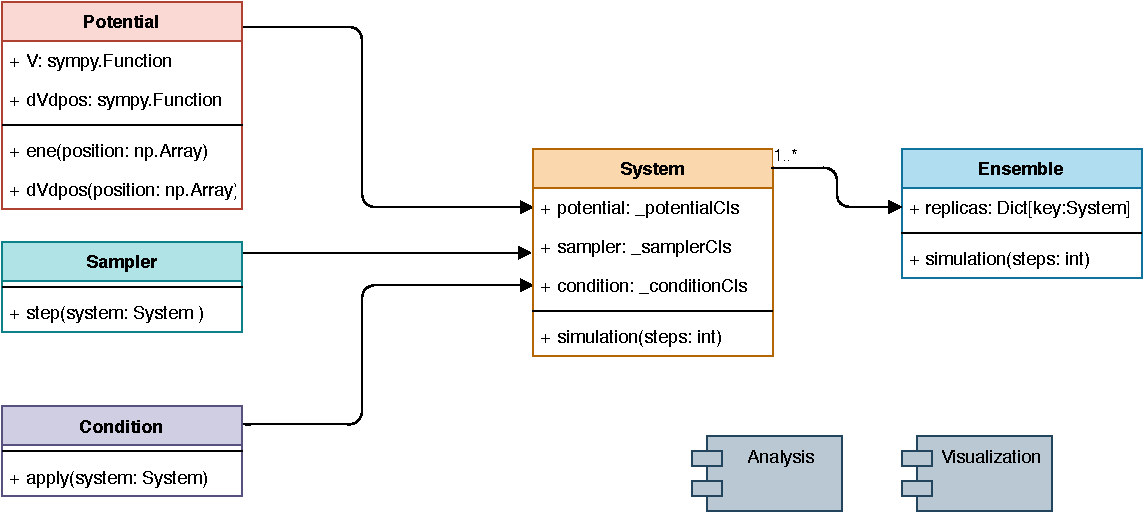
\includegraphics[width=\textwidth]{fig/implementation/export.pdf}
	\caption{Unified modeling language (UML) class diagram of the five Ensembler base classes. The \textit{potential class} defines the potential-energy functions to be explored and generates the required derivatives automatically (Figure \ref{fig:code_example_potential}). The implementation of a \textit{potential class} (red) is based on the symbolic mathematical language of SymPy.\cite{Meurer2017} The \textit{sampler classes} (cyan) are used for the sampling of potential-energy functions. \textit{Condition classes} (purple) can have different functions, e.g. application of periodic boundary conditions,\cite{Cheatham1995, Leach2001} thermostats, or restraints. The \textit{system classes} (orange) serve as the scaffold for the potential, sampler, and condition classes. In this structure, all components, parameters, and the results of a simulation are stored. The \textit{Ensemble class} (blue) can be used to perform advanced simulation techniques, e.g. using multiple walkers that explore the energy landscapes of the same or different systems as in replica-exchange approaches.\cite{Sugita1999, Sugita2000, Yamauchi2017} The \textit{analysis package} includes free-energy methods such as the Zwanzig equation\cite{Zwanzig1954} or BAR\cite{Bennett1976}. A set of visualization functions is provided in the \textit{visualization package} to enable an intuitive way of inspecting simulations or exploring potentials-energy functions. This includes plots, animations, and interactive widgets.}
	\label{fig:UML-Diagramm}
\end{figure}


%-------------------------------------------------------
\subsection{User level}
%-------------------------------------------------------
 A simulation model in Ensembler consists of a potential class, a sampler class, and a system class wrapping the potential and the sampler (Figure~\ref{fig:UML-Diagramm}), and provides control over the simulation approach. 
Additionally, multiple condition classes can be added that directly influence the simulation (e.g. periodic boundary condition\cite{Cheatham1995, Leach2001} or  thermostating\cite{Andersen1980}). 
After the construction of the system, the simulation can be started directly with the \textit{simulate} function. 
The resulting trajectory is in the form of a Pandas data frame.\cite{Mckinney2010} The trajectory is thus easily compatible with other packages like NumPy\cite{Vanderwalt2011} or scikit-learn\cite{Pedregosa2011} and can be stored in different formats, e.g. as .csv or .hf5 file. The system itself can be stored directly via the save function using serialization of the object with the Python package pickle.
In most cases, only a few additional lines are needed to go from simple simulation technique to more advanced one, as shown below. 

%-------------------------------------------------------
\subsection{Developer level}
%-------------------------------------------------------
The code of Ensembler is built on five interface-like base classes that allow extensive use of the inheritance concept and polymorphism \cite{Stroustrup1995} throughout the package.
These fundamental classes are \textit{potential}, \textit{sampler}, \textit{condition}, \textit{system}, and \textit{ensemble} (Figure \ref{fig:UML-Diagramm}), which can be grouped into three layers.
\textit{Potential}, \textit{sampler}, and \textit{condition classes} form the primary layer, providing different techniques to be used as components in a simulation. 
\textit{Potential classes} provide the potential-energy functions in a symbolic form using SymPy,\cite{Meurer2017} enabling automatic on-the-fly derivation and simplification of the potential-energy function. 
\textit{Sampler classes} are used to explore the potential-energy function (e.g. conjugate gradient,\cite{Hestenes1952} Metropolis MC,\cite{Hastings1970} or leap-frog\cite{Vangunsteren1988} integration). A new method can easily be implemented by inheriting from the \textit{sampler class} and overwriting a single function called \textit{step}. 
Finally, \textit{condition classes} provide additional functionalities such as thermostatting\cite{Andersen1980} and periodic boundary conditions\cite{Cheatham1995, Leach2001}). New techniques can be implemented by inheriting the base \textit{condition class} and overwriting the function \textit{apply}.
In the second layer, the first-layer components are wrapped into one \textit{system class} that executes the simulation(s) and manages the input and output. 
An optional higher-order layer is available in form of the \textit{ensemble class}, which allows the user to perform simulations with replica exchange.\cite{Sugita1999, Sugita2000, Yamauchi2017, Sidler2016}
If additional parameters are needed in a newly designed class, the constructor of the new child class can be adapted but must call the parent constructor.


%================================================================================
\section{Applications and Examples}
%================================================================================

%-------------------------------------------------------------------------------------------------------------------------
\subsection{Simple Simulations}
%-------------------------------------------------------------------------------------------------------------------------
In the following, simple code examples are shown to introduce the usage of Ensembler. In addition, an application example is provided to illustrate the use of Ensembler for teaching about free-energy methods. 
The code for these examples can be found in the GitHub repository \textit{\hyperlink{https://github.com/rinikerlab/Ensembler}{https://github.com/rinikerlab/Ensembler/examples}}.
\begin{figure}[h!]
	\centering
	\begin{subfigure}{0.85\textwidth}
		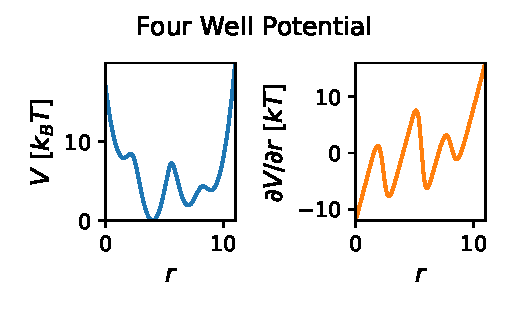
\includegraphics[width=\linewidth, height=1.75in]{fig/codeExamples/four_well.pdf} 
		\caption{}
	\end{subfigure}\\
	\begin{subfigure}{0.85\textwidth}
		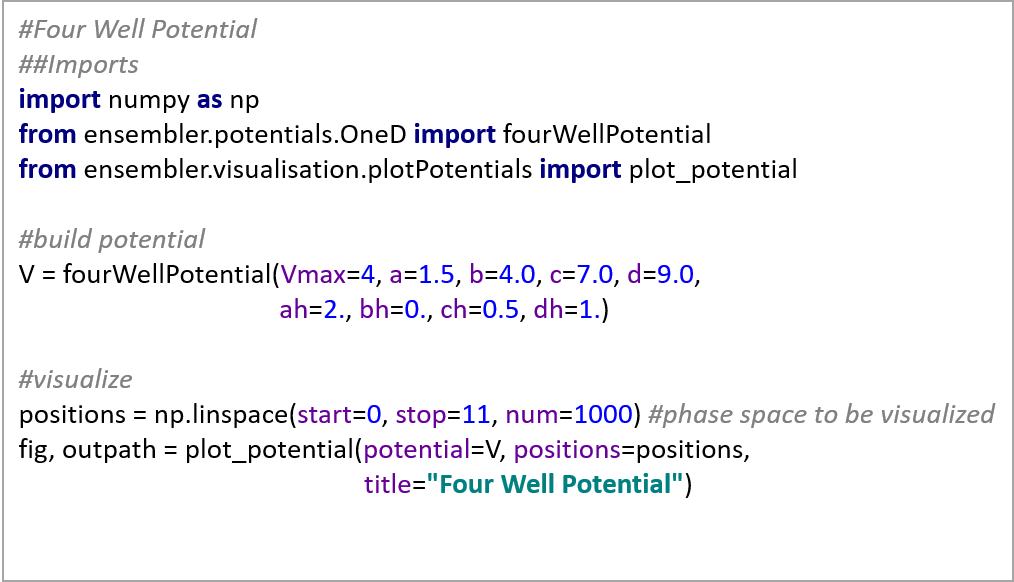
\includegraphics[width=\linewidth, height=1.75in]{fig/codeExamples/Potential_code.png}
		\caption{}
	\end{subfigure}
	\caption{A four-well potential-energy surface visualized by the standard visualization function of Ensembler. (a) Potential-energy function (blue) and the automatically generated spatial gradient (orange) over a given coordinate range. (b) Source code to define the potential-energy function and the coordinate range to be visualized. These parameters are passed to the built-in plotting function in the \textit{potential classes} of Ensembler.}
	\label{fig:code_example_potential}
\end{figure}

In typical applications of Ensembler, the user selects a potential-energy function from the available ones. In the following example, a potential-energy function with four wells is selected and initialized with chosen parameters. 
To sample this four-well potential-energy function with stochastic dynamics (SD),\cite{Brunger1984} the sampling method is instantiated and passed to the \textit{system class}, which controls the execution of the simulation. 
The simulation is performed by calling the function \textit{simulate} with the desired number of simulation steps passed as parameter. 
Subsequently, the results can be visualized using the built-in visualization functions that are compatible with the \textit{simulation class} of Ensembler.  
As can be seen in Figure \ref{fig:code_example_simulations}a, the energy barriers between the different minima were not crossed during the chosen simulation length. 
To overcome the sampling issue, enhanced sampling techniques can be employed.\cite{Pohorille2010} 
In this example, local elevation\cite{Huber1994}/metadynamics\cite{Laio2002} is used to overcome the energy barriers (Figure \ref{fig:code_example_simulations}b).
The method adds a time-dependent biasing potential to the system, i.e. it adds a Gaussian biasing potential to positions that were already visited such that they become energetically less favorable. This decreases the likelihood of visiting known positions again. 
The enhanced sampling technique can be applied by adding a single line of code compared to the previous simulation (Figure \ref{fig:code_example_simulations}c).

\begin{figure}[h]
	\centering
	\begin{subfigure}{\textwidth}
		\caption{Standard Langevin Simulation}
		\centering
		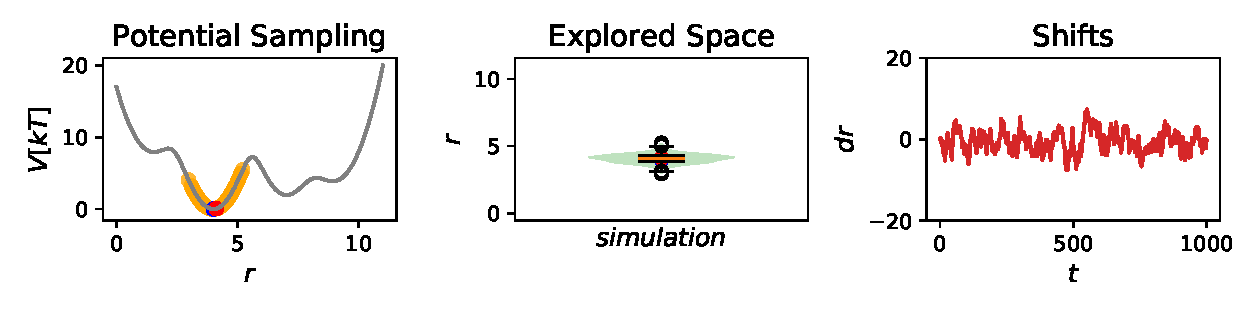
\includegraphics[width=0.85\linewidth]{fig/codeExamples/langevin_simulation.pdf} 
	\end{subfigure}
	\vspace{2.5mm}
	\begin{subfigure}{\textwidth}
		\caption{Langevin Simulation with Local Elevation/Metadynamics}
		\centering
		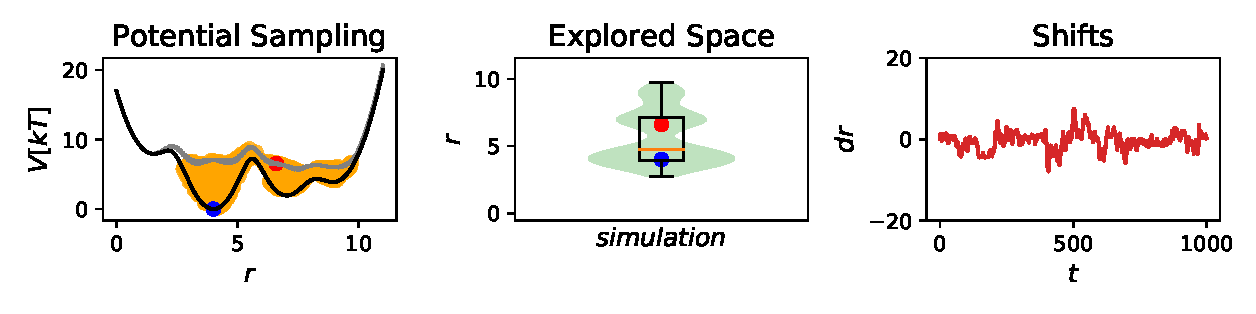
\includegraphics[width=0.85\linewidth]{fig/codeExamples/metaDynamics_simulation.pdf}
	\end{subfigure}
	\vspace{2.5mm}
	\begin{subfigure}{\textwidth}
		\caption{Example Source Code}
		\centering
		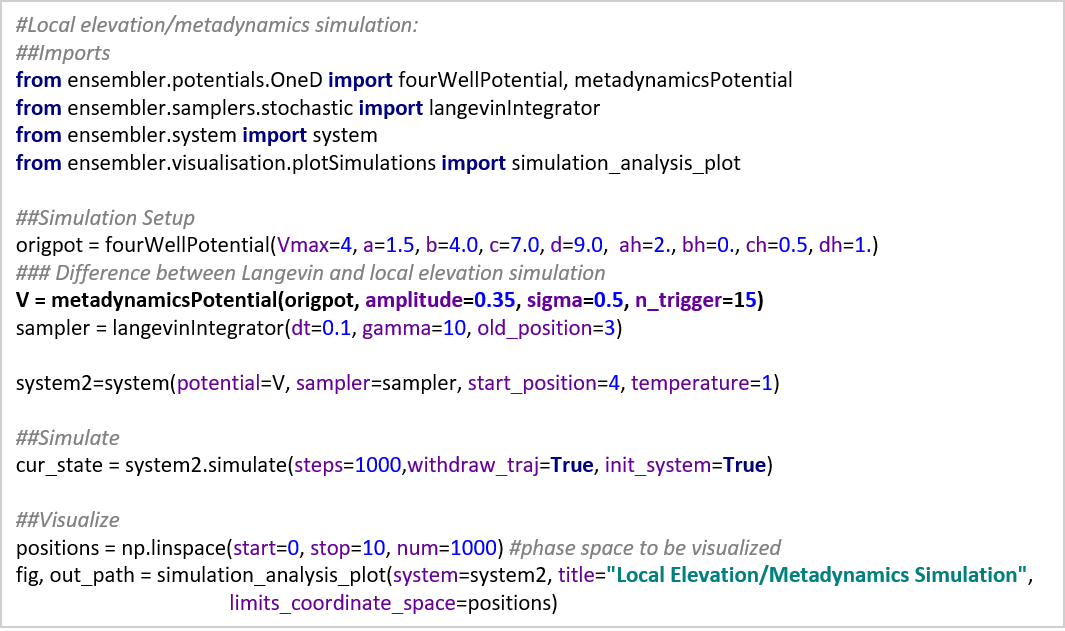
\includegraphics[width=0.85\linewidth]{fig/codeExamples/Simulation_code.png}
	\end{subfigure}
\caption{Langevin simulation of a four-well potential energy-function. Results when sampling (1000 steps) with the standard SD integrator (a) or with local elevation\cite{Huber1994}/metadynamics\cite{Laio2002} (b). The left panel shows the potential-energy surface (black), the sampled range (orange), as well as the start point (blue) and end point (red). The middle panel shows the sampled space as a violin/box plot with the start point (blue) and end point (red). The right panel shows the shift $\Delta r_t$ = $r_{t+1}$ - $r_t$ as a function of simulation time $t$.
	(c) Source code to perform the simulations. First, the four-well \textit{potential class} and the Langevin \textit{sampler class} are initiated. Next, they are wrapped by a \textit{system class}, which executes the simulation. Visualizations are generated with a built-in functions. Note that only one line has to be added to use the enhanced sampling technique (marked in bold).}
\label{fig:code_example_simulations}
\end{figure}

\FloatBarrier
\clearpage

%-------------------------------------------------------------------------------------------------------------------------
\subsection{Free-Energy Calculation}
%-------------------------------------------------------------------------------------------------------------------------

Free-energy calculation is an important field in computational chemistry because free-energy differences govern the outcome of processes in nature, e.g. protein-ligand binding or polymer formation.\cite{Christ2009, Hansen2014, Cournia2020, Armacost2020} 
%
The calculation of alchemical free-energy differences with Ensembler is exemplified with a mutation of the equilibrium position of a one-dimensional harmonic oscillator (Figure \ref{fig:FE_sampling}a).
This mutation corresponds to a change of a covalent bond type at the terminus of a linear molecule and can be calculated analytically (Table \ref{tab:FE_results}).
In practical applications, however, it is usually not possible to calculate the free-energy difference analytically. In these cases, MD-based simulation techniques can be employed.
In the following, the sampling of the two end states of the model system and the results of the free-energy calculation with different methods are discussed. For more details, we refer to the Jupyter notebook in the Ensembler GitHub repository.

A simple free-energy method is to simulate one end state and estimate the free-energy difference with the Zwanzig equation.\cite{Zwanzig1954} The quality of the result depends on a sufficient phase-space overlap between the two end states.\cite{Konig2018}
Alternatively, one can simulate both end states separately and use BAR\cite{Bennett1976} (Figure \ref{fig:FE_sampling}a), yielding more converged results.\cite{Konig2018}
If the phase-space overlap between the two end states is not sufficient, more advanced sampling methods are necessary to obtain converged free-energy differences.
%
\begin{figure}[h]
	\centering
	\begin{subfigure}{.85\textwidth}
		\caption{}
		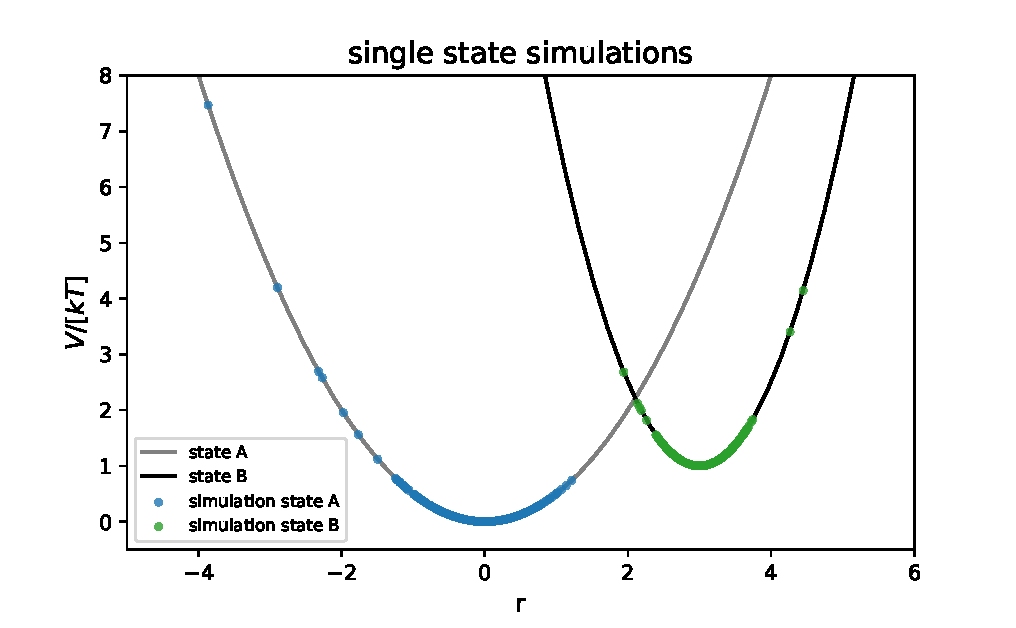
\includegraphics[width=\linewidth]{fig/FE_example/freeEnergyPertubation.pdf} 
	\end{subfigure}\\
	\begin{subfigure}{.85\textwidth}
		\caption{}
		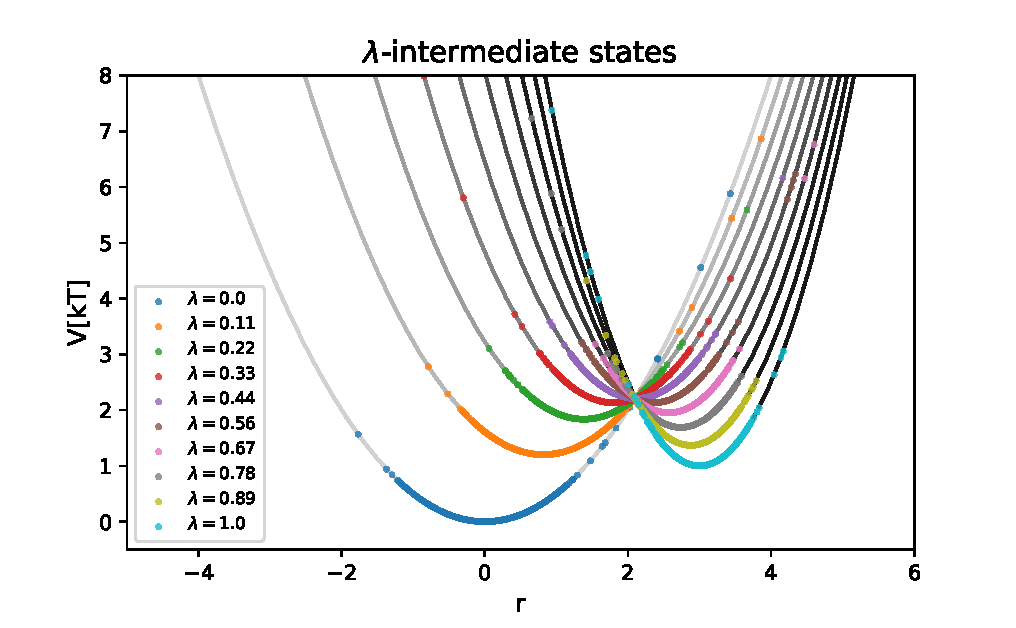
\includegraphics[width=\linewidth]{fig/FE_example/linear_coupled.pdf} 
	\end{subfigure}
	\caption{Illustration of different free-energy methods implemented in Ensembler (part I). (a) For FEP\cite{Zwanzig1954} and BAR\cite{Bennett1976}, the two end states (grey and black) are sampled separately (green and blue). (b) To increase the phase-space overlap, the two end states can be coupled as a linear combination of their Hamiltonians using a coupling parameter $\lambda$. This allows the generation of intermediate states (grey to black) and sampling of those (colored points).}
	\label{fig:FE_sampling}
\end{figure}
%
\begin{figure}[h]
	\centering
	\begin{subfigure}{.85\textwidth}
		\caption{}
		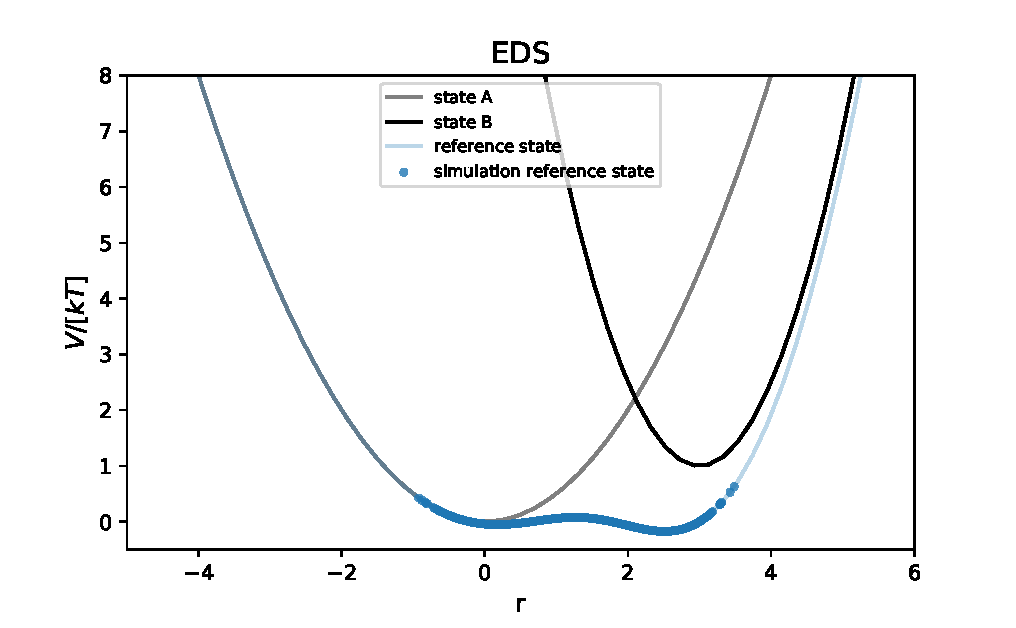
\includegraphics[width=\linewidth]{fig/FE_example/EDS_sampling.pdf} 
	\end{subfigure}\\
	\begin{subfigure}{.85\textwidth}
		\caption{}
		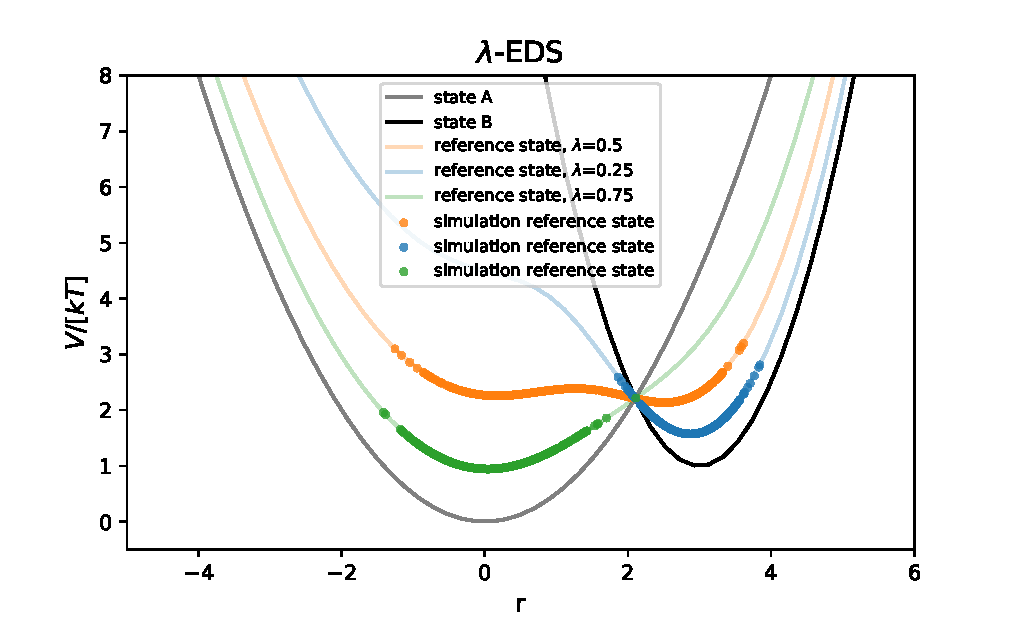
\includegraphics[width=\linewidth]{fig/FE_example/hlEDS_sampling.pdf} 
	\end{subfigure}
	\caption{Illustration of different free-energy methods implemented in Ensembler (part II). (a) An alternative method is EDS,\cite{Christ2007, Christ2008, Christ2009} where a reference-state Hamiltonian (blue line) is sampled (blue points), which envelopes the end states. By setting the reference-state parameters to $s$~=~0.3 and energy offsets~=~[0,0], all relevant phase-space regions can be sampled. (b) A recently developed approach called $\lambda$-EDS\cite{Koenig2020} introduces a $\lambda$-dependence in the EDS method (blue, orange and green line). Colored points indicate sampling. The reference-state parameters were set to $s$~=~0.3 and energy offsets~=~[0,0], and three different lambda values 0.25,0.5, 0.75 were chosen.}
	\label{fig:FE_samplingb}
\end{figure}
%%linear coupling
One possibility to increase the phase-space overlap is to generate intermediate states as a linear combination of the two end states $A$ and $B$ with the coupling parameter $\lambda$, i.e. $H(\lambda) = (1-\lambda) H_A + \lambda H_B$, such that $H(\lambda=0) = H_A$ and $H(\lambda=1) = H_B$.
The intermediate states are positioned at discrete $\lambda$-points between 0 and 1 (Figure \ref{fig:FE_sampling}b).\cite{Valleau1972, Straatsma1991} 
The free-energy difference can be estimated using FEP\cite{Zwanzig1954} or BAR\cite{Bennett1976} as the path over all intermediates, or with TI\cite{Kirkwood1935} as the integral along $\lambda$. 

%% EDS
Another elegant free-energy method is EDS,\cite{Christ2007, Christ2008} where a reference-state Hamiltonian $H_r$ is sampled. $H_r$ is constructed as a log-sum of the Hamiltonians of the two (or more) end states, guaranteeing the phase-space overlap of the reference state with all end states,
\begin{equation}
H_R = - \frac{1}{\beta s} \ln( e^{(- \beta s (H_A - E^R_A)}) +e^{(- \beta s (H_B - E^R_B)}),
\end{equation}
where $1/\beta=k_{B}T$, $k_B$ being the Boltzmann constant and $T$ the absolute temperature.
$H_R$ can be optimized for sampling using two kinds of parameters: The smoothing parameter $s$ lowers the energy barriers between the end states, whereas the energy offsets $E^R$ ensure equal weighting of all end states. In our example, both end states are sampled sufficiently during the EDS simulation with $s=0.3$ and the energy offsets $E^R=[0,0]$ (Figure \ref{fig:FE_sampling}c). Subsequently, the Zwanzig equation\cite{Zwanzig1954} is used to obtain the free-energy difference between the end states.\cite{Christ2007, Christ2008}
%hybrid coupling l-EDS
Recently, a hybrid form of EDS and $\lambda$-coupling was introduced, termed $\lambda$-EDS.\cite{Koenig2020} At $\lambda=0$ or $1$, the $H_R$ is equal to the Hamiltonians of the respective end states, while conventional EDS is recovered with $\lambda$=0.5 (except for an offset).\cite{Koenig2020}
$\lambda$-EDS allows for a $\lambda$-weighting of the exponential terms in the EDS equation. In the example in Figure \ref{fig:FE_sampling}d, the same reference-state parameters were used as before.

%final comparison
All free-energy calculations discussed above were performed with Ensembler for a total of 10'000 Monte Carlo (MC)\cite{Hastings1970} steps, and each simulation was repeated five times.
The simulation results listed in Table \ref{tab:FE_results} show that larger errors are obtained without intermediate states due to insufficient phase-space overlap.
Using ten $\lambda$–intermediate states together with TI gave the best result, however, this approach is also the computationally most expensive one (i.e. ten separate simulations). s
EDS and $\lambda$-EDS, on the other hand, yielded also good results, while requiring only one simulation (given a set of suitable reference-state parameters). 
We refer to the Jupyter notebook in the Ensembler GitHub repository for the source code, more detailed information on these methods as well as additional methods like conveyor-belt TI\cite{Hahn2019} and RE-EDS,\cite{Sidler2016, Sidler2017} which combine enhanced sampling and free-energy methods.
\begin{table}[ht]
	\centering
	\caption{Estimated free-energy difference for the model system shown in Figure \ref{fig:FE_sampling}. Sampling was performed with Monte Carlo method (MC)\cite{Hastings1970} for 10'000 steps in each simulation. Each calculation was replicated five times and the averaged result is shown together with the standard deviation.
		The duration of the computations (without visualizations) was estimated directly in the Jupyter notebook and is given relative to the FEP simulation (absolute duration = 2.0 seconds). The performance was tested on a Lenovo Thinkpad T420s with an Intel i5-2520 ($2.5~\text{GHz}$) CPU and $8~\text{GB}$ RAM. The RAM usage for the full Jupyter notebook execution was in total $578~\text{MB}$.}
	\label{tab:FE_results}
	\resizebox{\columnwidth}{!}{%
		\begin{tabular}{l|r | c| r r}
			Method & Average $\Delta$F & Deviation from & \multicolumn{2}{c}{Speed (rel. to FEP)}\\
			&      [$k_B T$]  & analytical result [$k_B T$] & Simulation & Analysis \\
			\hline
			\textit{analytical} & 1.275 & - & - & -  \\
			FEP\cite{Zwanzig1954} & $6.579 \pm  1.009$ & 5.305 & 1.0 & 0.1  \\
			BAR\cite{Bennett1976} & $2.437 \pm  0.500$ & 2.437 & 3.0 & 2.1 \\
			FEP 10-$\lambda$-points &  $1.406 \pm 0.431$ & 0.131 & 14.0 & 0.7 \\
			TI\cite{Kirkwood1935} 10-$\lambda$-points& $1.242 \pm 0.015$ & 0.033 & 14.0 & 0.04\\
			EDS\cite{Christ2007, Christ2008, Christ2009} &  $0.958 \pm 0.110$ & 0.317 & 2.4 &  0.2 \\
			$\lambda$-EDS\cite{Koenig2020} $\lambda=0.5$ & $ 0.987 \pm  0.111$ & 0.287 & 3.1 & 0.2\\
		\end{tabular}
	}
\end{table}


\clearpage
\newpage

%================================================================================
\section{Conclusion}
%================================================================================

In the present chapter, we proposed a new method called 
conveyor belt thermodynamic integration (CBTI)
to calculate alchemical free-energy differences based on 
MD simulations.
%
This approach borrows and combines ideas from
thermodynamic integration\cite{KI33.1,KI34.2,KI35.1} (TI),
\radd{replica exchange\cite{SU99.1,FU02.2,ZH16.2} (HRE) or permutation\cite{IT13.1,IT13.2,YA17.2} (HRP),}
and $\lambda$-dynamics\cite{KO96.1,DA01.7,GU03.1,KN09.1,KN11.2,DO11.2,AR15.2,HA17.1} ($\lambda$D),
along with the real-life working principle
of the funicular.
%

%
In CBTI, one simulates in parallel a set of $K$ 
\radd{equally spaced} replicas
(with $K$ even) on a forward-turn-backward-turn 
path along the alchemical coupling variable $\lambda$, 
akin to a conveyor belt (CB) between the two physical end 
states.
%
Because the $\lambda$-forces (Hamiltonian $\lambda$-derivative)
exerted by the individual replicas on the CB largely 
compensate each other, the overall $\Lambda$-force on 
the CB advance variable $\Lambda$ becomes increasingly 
small when $K$ is made increasingly large (residual free-energy
barriers decreasing at least as $K^{-1}$ \radd{in the limit of large $K$}, as shown in \refsec{quad}).
%
As a result, \radd{for a sufficient number $K$}, quasi-homogeneous
sampling of the $\lambda$-range can be achieved
without application of any biasing potential.
%
If a \radd{smaller $K$} is employed, a memory-based biasing potential 
can still be added to further homogenize the sampling,
the preoptimization of which is computationally inexpensive.
%
The results of a CBTI simulation (whether biased or not) can be analyzed similarly to TI,
by binning of the \radd{average} Hamiltonian $\lambda$-derivative as a function 
of $\lambda$ considering all replicas jointly, followed 
by quadrature integration. 
%
In this case, the continuous and quasi-homogeneous sampling of the $\lam$-range permits to use a large number of bins,
thereby essentially eliminating quadrature errors.

As a first application, 
the CBTI scheme was employed here to calculate the 
hydration free energy of methanol.
%
It was shown that the method is rather robust with respect 
to the choice of its parameters ($K$ as well as the mass-parameter $m_{\Lamb}$ and thermostat coupling time $\tau_\Lamb$ of the CB), the 
most important sensitivity being relative to $K$.
%
Upon increasing $K$, the distribution/dynamics of $\Lambda$ evolves 
from regularly spaced preferential values with a hopping dynamics
to quasi-homogeneous coverage with a diffusive dynamics.
%
For the smallest number of replicas considered ($K=8$), application 
of a biasing potential is recommended. For larger numbers of 
replicas ($K\ge 16$), it becomes unnecessary.
%
The calculated $\Delta G$ values compare well with those obtained using other methods.




The convergence is accelerated relative to TI with Simpson quadrature (smaller error bar at identical
total single-system sampling time), owing to improved orthogonal sampling and reduced quadrature errors.
It is comparable to HRE, which shares the same orthogonal-sampling advantage.
\revphil{
It is also similar to TI with EXTI or MBAR as free-energy estimator,
which achieve a similar improvement {\em via} an orthogonal-statistics advantage,
{\em i.e.} by effectively mixing information concerning distinct configurational 
wells across $\lambda$-points.
}
%One might refer to these two types of effects
%orthogonal-sampling {\em vs.} orthogonal-statistics
%advantages, respectively.
%
%. However, the TI-like
%\philrev{The free-energy estimator employed here for CBTI may nevertheless
%still be sub-optimal in terms of statistical efficiency relative to \eg{} EXTI and MBAR.}
%
%
\revphil{It should be stressed, however, 
that the present mutation
is rather non-challenging in terms of orthogonal sampling.
%, {\em i.e.} we expect a 
%simple unimodal conformational behavior in the orthogonal space at each $\lambda$-value.
%
Work is in progress to investigate other types of systems with more complicated
%difficult
%"challenging" 
orthogonal spaces:
($i$) the side-chain mutation in the central residue of a tripeptide considered in Refs.~\citenum{BI15.1,GR16.4};
($ii$) the hydrogen-to-bromine mutation in the base of a 
%flexible 
nucleotide considered in Refs.~\citenum{HR08.1,HR09.1,GA13.4}.
%
Here, it is expected that CBTI alone (just like HRE)
will help overcoming 
%high 
barriers in the orthogonal space
when these barriers are low at some $\lambda$-value
(as in the first system mentioned),
but may be insufficient on its own when these barriers
are high at all $\lambda$-values (as in the second system mentioned),
in which case additional modifications must be applied to create artificially 
an orthogonal tunnel at least over a limited $\lambda$-range.
}


Compared to existing MD-based alchemical free-energy calculation methods, the CBTI scheme can be viewed in at least three different ways:
%
($i$) as a \radd{continuous/deterministic/dynamical}
%dynamical 
(instead of discrete/stochastic) analog 
of the HRE scheme\cite{SU99.1,FU02.2,ZH16.2} or the HRP scheme\cite{IT13.1,IT13.2,YA17.2};
($ii$) as a correlated multiple-replica analog (reminiscent of other swarm\cite{HU98.6,BU15.5,KA18.6,AL18.2}, multiple-walker\cite{RA06.2,CO14.5} or flying-Gaussian\cite{SU16.3,KR17.1} approaches)
       of the $\lambda$-local elevation umbrella sampling ($\lambda$-LEUS) scheme\cite{BI14.1,BI14.2,BI15.1,BI15.2} (or the conceptually similar flat-histogram\cite{WA01.5,LA04.6}
       $\lambda$-metadynamics\cite{LA02.1,BA08.2,WU11.1}, adaptive integration\cite{FA04.3}, adaptive biasing force\cite{DA08.2}, \radd{adaptively biased\cite{BA08.1} and} expanded-ensemble\cite{LY92.1,LY94.1,LY96.2,ES07.1,ES07.2,PA11.7,RA18.2} methods);
       ($iii$) as an equilibrium multiple-replica variant of the slow-growth\cite{BE85.3,ST86.1} (SG) method (bypassing the associated hysteresis issues\cite{PE89.1,HE91.1,MA94.12} or the requirement for
       exponential averaging over multiple repeats\cite{JA97.3,CR00.2,HE01.4,HU02.2}).
       %
       
%
Compared to plain TI, it shares the advantage of HRE/HRP and $\lambda$-LEUS
in terms of enhanced orthogonal sampling\cite{WO03.1,WO03.2,KH10.1,KH11.2}.
%
Compared to HRE/HRP, it permits a deterministic and continuous sampling
of the $\lambda$-range, and bypasses the need for a careful preselection\cite{KO05.8,RA05.8,TR06.5,SI08.3,NA08.6,VO15.2,VO15.3,ZH16.2,SU17.3,MA18.8}
of the $\lambda$-ladder and exchange-attempt interval.
%
Compared to both TI and HRE/HRP, the quasi-homogeneous $\lambda$-sampling 
also essentially removes quadrature errors.
%
Finally, compared to $\lambda$-LEUS, it eliminates (or drastically reduces) 
the dead time associated with the preoptimization of a biasing potential\cite{BI14.1}
or, alternatively, the use of this formally non-equilibrium statistics\cite{HA10.1} 
in the production calculation\cite{BA08.2}.
%
%%%
For the above reasons, the CBTI scheme certainly represents a
%very 
useful addition to the alchemical free-energy calculation toolkit.


\revphil{Like TI and HRE/HRP, the CBTI method is also intrinsically parallel.
%
However, assuming that the replicas are assigned to separate processors 
(including possible GPU implementations or/and cloud-computing applications),
the requirement of an all-to-all information exchange between processors
at every timestep might represent a drawback of the method relative to the no-exchange
and infrequent exchange situations of TI and HRE/HRP, respectively.
%
Although the communication is lightweight (Hamiltonian $\lambda$-derivative,
{\em i.e.} a single real number), the synchronization requirement may cause 
a performance loss (reduced scalability and fault tolerance).
%
Unless asynchronous variants\cite{GA15.12,XI15.7} or multiple-timestep schemes\cite{MO11.3,MA16.24} can be developed,
this performance loss may represent a problem for parallel applications
in situations involving many replicas of a small system, as these will
involve more data exchange at a more frequent rate.
%
}


%
%
%
This scheme opens the way to at least two types of generalizations and extensions.
%
%
%
%
First, a number of components of the scheme can be modified/generalized and in particular the following:
%
($i$) different functions $\zeta$ may be used \radd{in \refeq{cb_lam_of_big_lam}}
%\refeq{zigzag_fct}
      to modulate the replica density along $\lambda$ ({\em e.g.} smoothing the tips
      or adding plateaus\cite{BI14.1} for a denser sampling
      close to or at the physical end-states);
%
($ii$) different matrices $\Cmat$ may be used in \refeq{cb_def} corresponding to
       a to non-uniform weighting of the $\lam$-forces into the $\Lamb$-force,
       ({\em e.g.} canceling the effect of higher-order
       derivatives by alternating non-integer weights in analogy to standard quadrature methods);
($iii$) the coupling between replicas may be generalized
        from sequential pairwise constraints to possibly non-pairwise potentials
        (\eg{} collective or harmonic);
($iv$) the TI-like free-energy estimator of \refeq{cbti_formula} may be replaced by
          a statistically more powerful one of the MBAR
%/UWHAM/RBE 
type\cite{LU04.3,SH05.6,SH08.7,FA09.4,TA12.1,DI17.5,ZH17.6};
($v$) CBTI would benefit from the use of an alchemical coupling path
          presenting a vanishing free-energy derivative at the physical end-states (residual free-energy 
          barriers along $\Lamb$ decaying at least in $K^{-2}$ instead of $K^{-1}$ \radd{for large $K$}, as shown in \refsec{quad}).



Second, the application range of CBTI, restricted here to alchemical processes,
can be extended to encompass either thermodynamic or conformational free-energy 
changes.
%
In the former case, extension to a CB \radd{variant of} parallel \radd{tempering\cite{SU99.1} ({\em i.e.} a CBPT scheme)}
appears relatively straightforward considering that scaling the temperature
is equivalent to scaling the system potential energy. 
Such a 
%\revdavid{[DELETE?: CBTI] 
CBPT scheme would represent a form of
\revphil{multicanonical} \radd{sampling\cite{BA87.2,BE91.6,BE92.1}}.
%
%          *** BA87.2  : [Baumann] Noncanonical path and surface simulation.
%          > early ref, has the basic idea of non-canonical weight factors (but BE92.6 and BE92.1 are probably more to the point)
%          *** BE91.6  : [Berg/Neuhaus] Multicanonical algorithms for first order phase transitions.
%          > I think they use an approximate parametrized (one-param) fct to represent the density of states
%          > Phase transition in a lattice (Potts) model
%          *** BE92.1  : [Berg/Neuhaus] Multicanonical ensemble: A new approach to simulate first-order phase transitions.
%          > Similar
%
In the latter case, extension to a CB \radd{variant of} umbrella \radd{sampling\cite{TO74.1,TO77.1} ({\em i.e.} a CBUS scheme)}
could be designed {\em e.g.} by anchoring harmonic potentials to the CB
and propagating the corresponding restraining forces onto the CB.
%
Finally the extension of the CB approach to multistate problems\cite{KN11.2,BI15.2,HA17.1,VI18.2} 
({\em e.g.} path or network of CBs connecting the different states of a system)
as well as multidimensional problems (sub-CBs anchored to a main CB) can also
be envisioned.


\clearpage
\pagebreak


%\bibliography{3_chapter_1/ref/ref.bib}

\end{document}
